\section{Ergebnisse}

\begin{frame}\frametitle{Inhalt}
	\tableofcontents[currentsection,hideallsubsections]
\end{frame}

\subsection{Zeitdiskretes Survival-Modell}

\begin{frame}\frametitle{Optimale Iterationsanzahl}
	\centering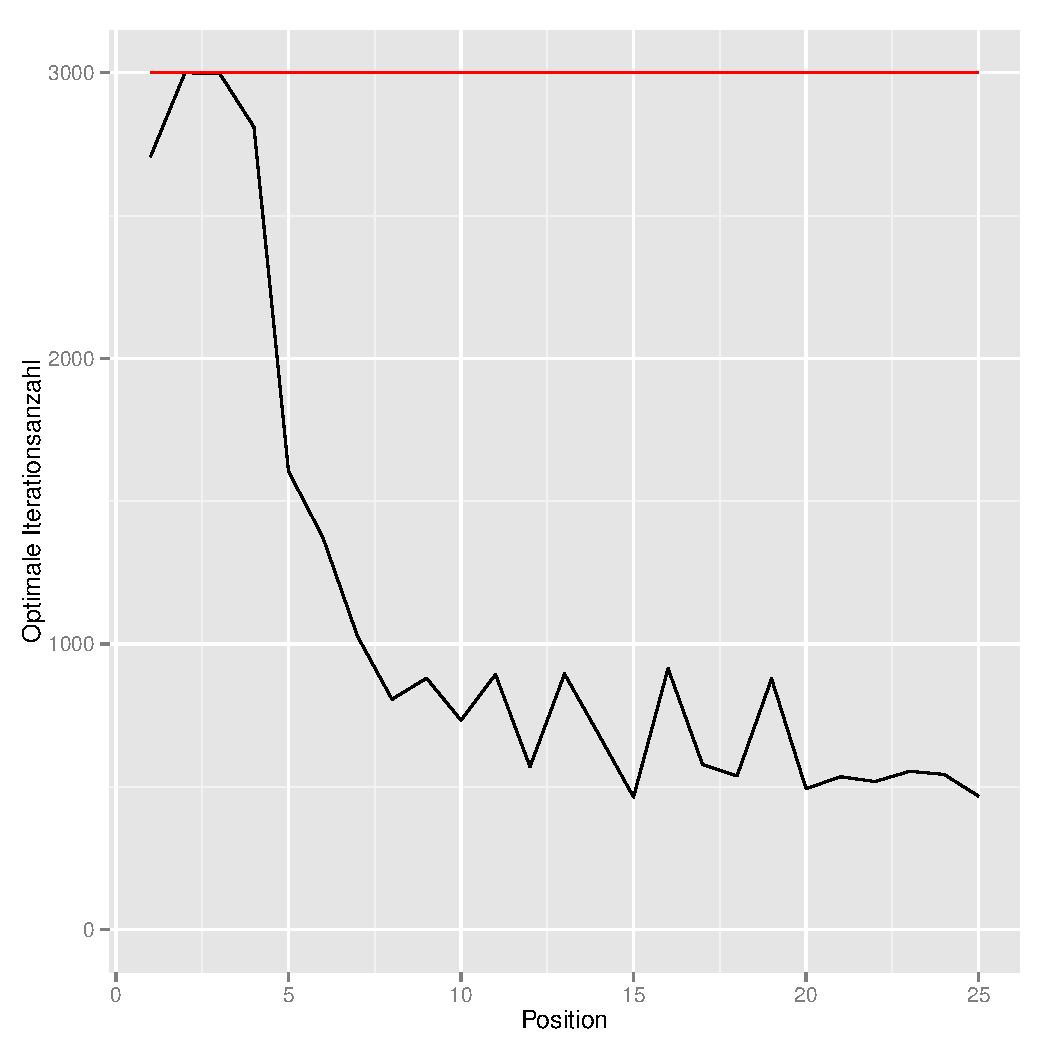
\includegraphics[scale=0.3]{bestIter.pdf}
\end{frame}

\begin{frame}\frametitle{Relative Wichtigkeit der Features}
	\centering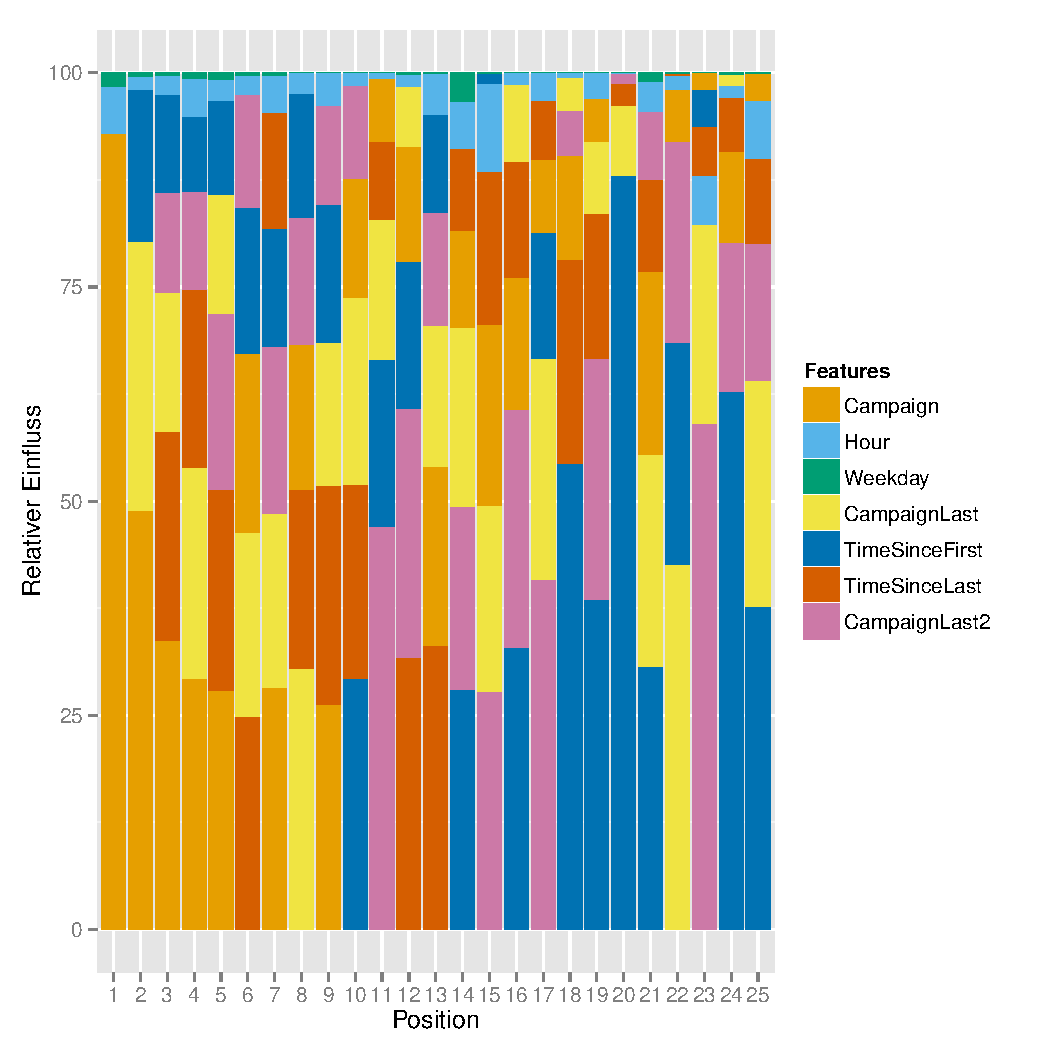
\includegraphics[scale=0.3]{variableImportance.pdf}
\end{frame}

\begin{frame}\frametitle{Marginale Effekte - campaign}
	\centering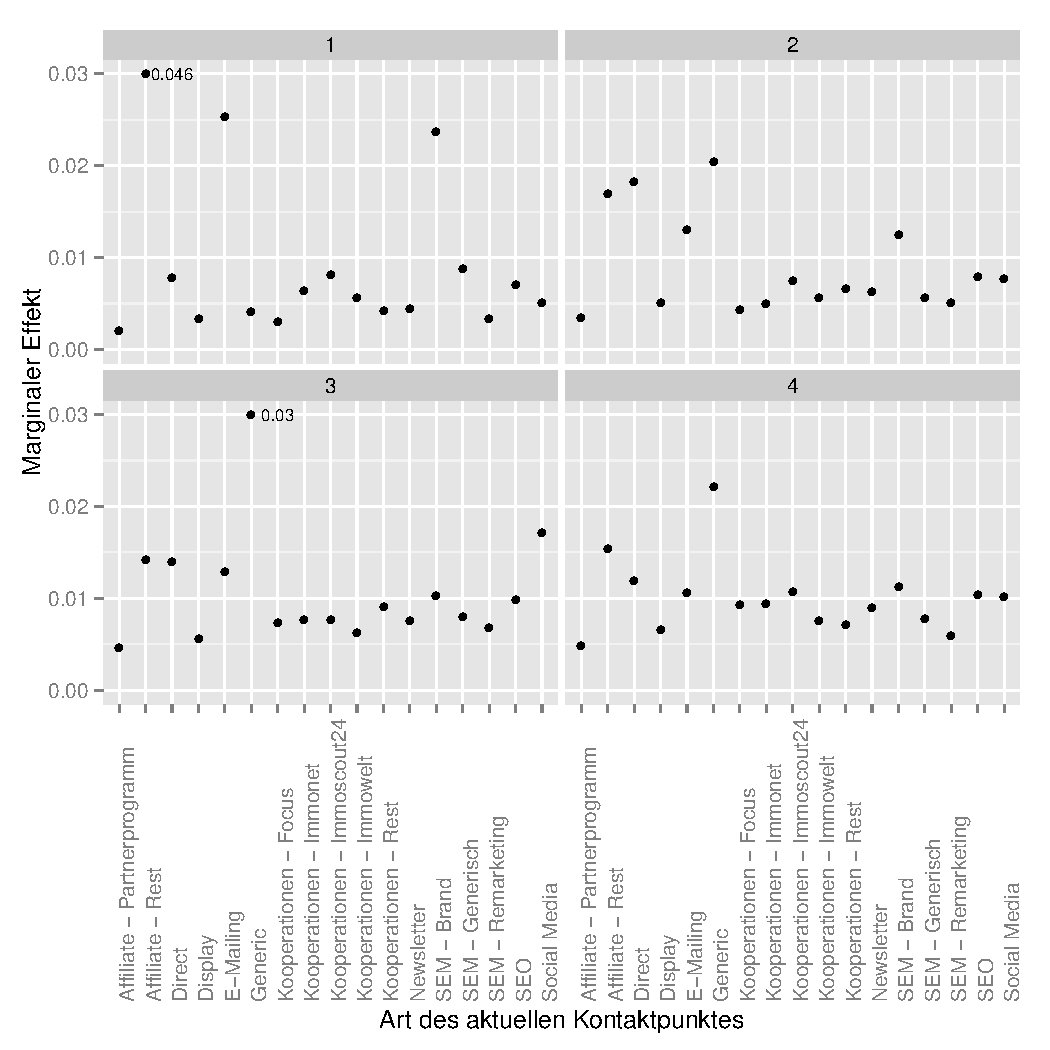
\includegraphics[scale=0.3]{marg_eff_campaign.pdf}
\end{frame}

\begin{frame}\frametitle{Marginale Effekte - campaignLast}
	\centering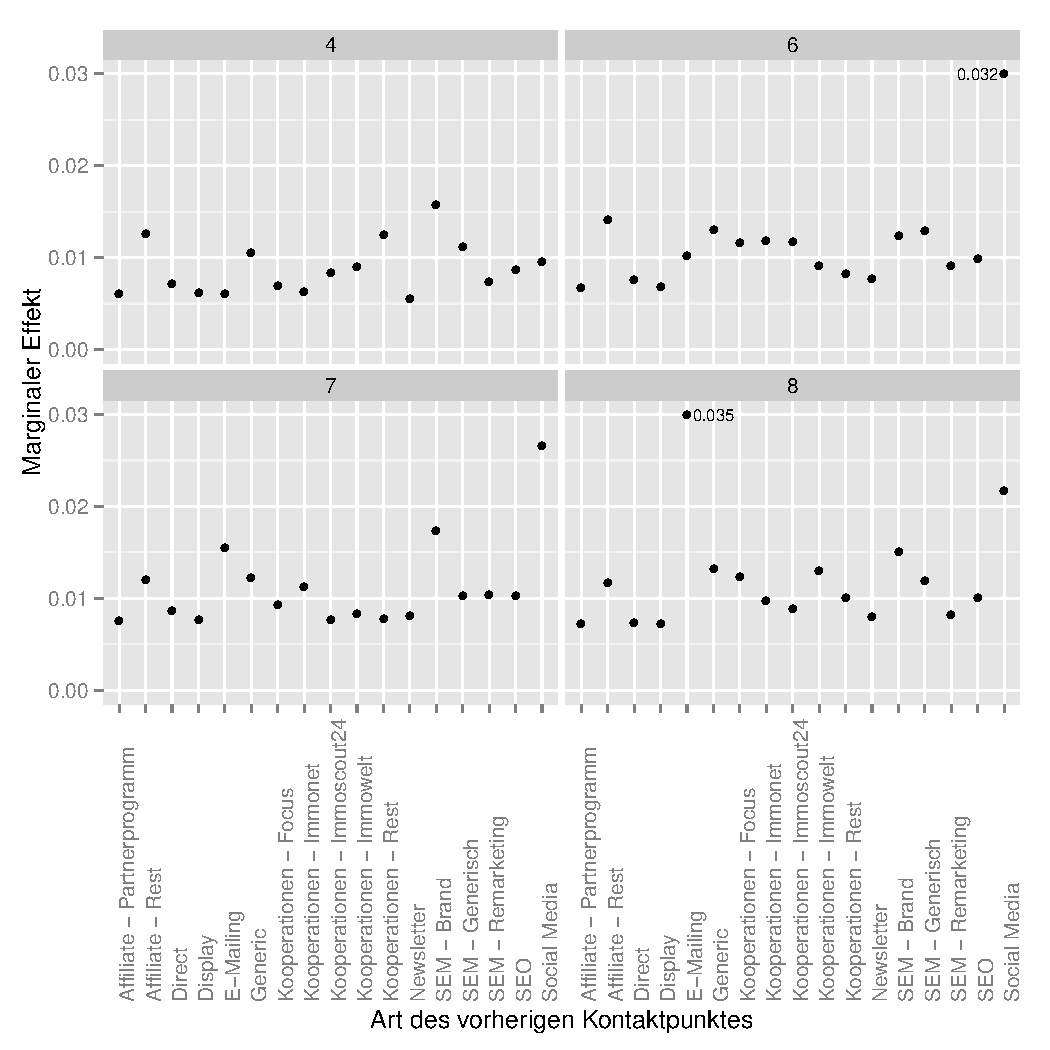
\includegraphics[scale=0.3]{marg_eff_campaignLast.pdf}
\end{frame}

\begin{frame}\frametitle{Marginale Effekte - timeSinceFirst \& timeSinceLast}
	\centering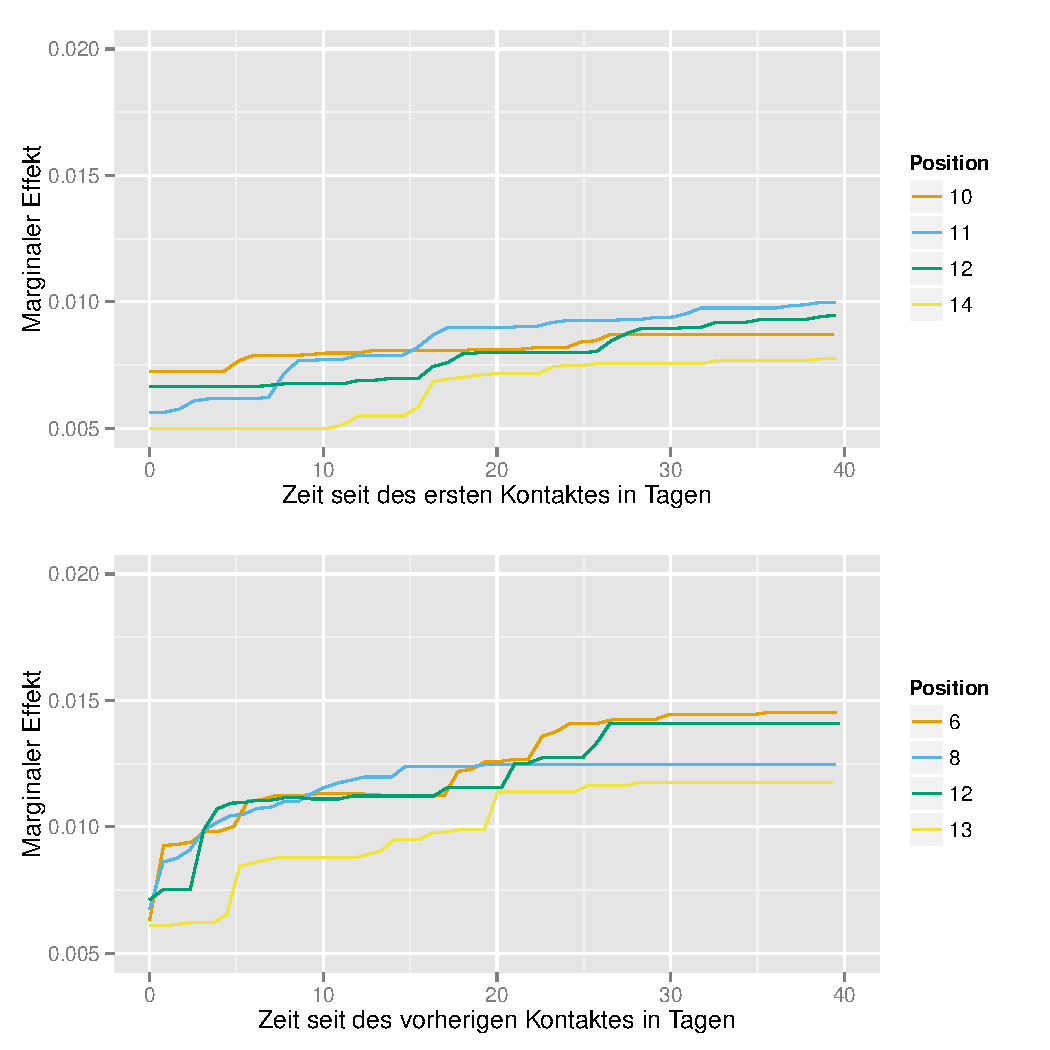
\includegraphics[scale=0.3]{marg_eff_time.pdf}
\end{frame}

\begin{frame}\frametitle{ROC-Kurve}
	\centering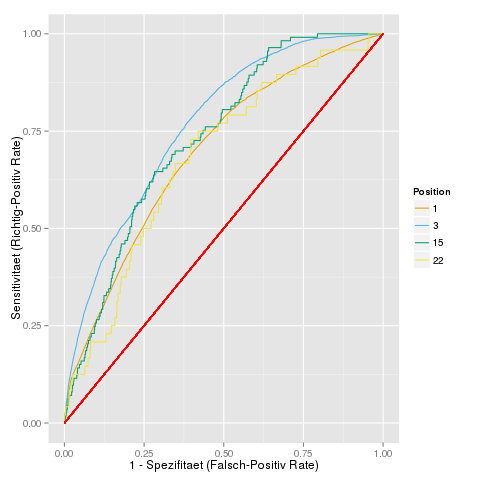
\includegraphics[scale=0.3]{roc.png}
\end{frame}

\begin{frame}\frametitle{AUC}
	\centering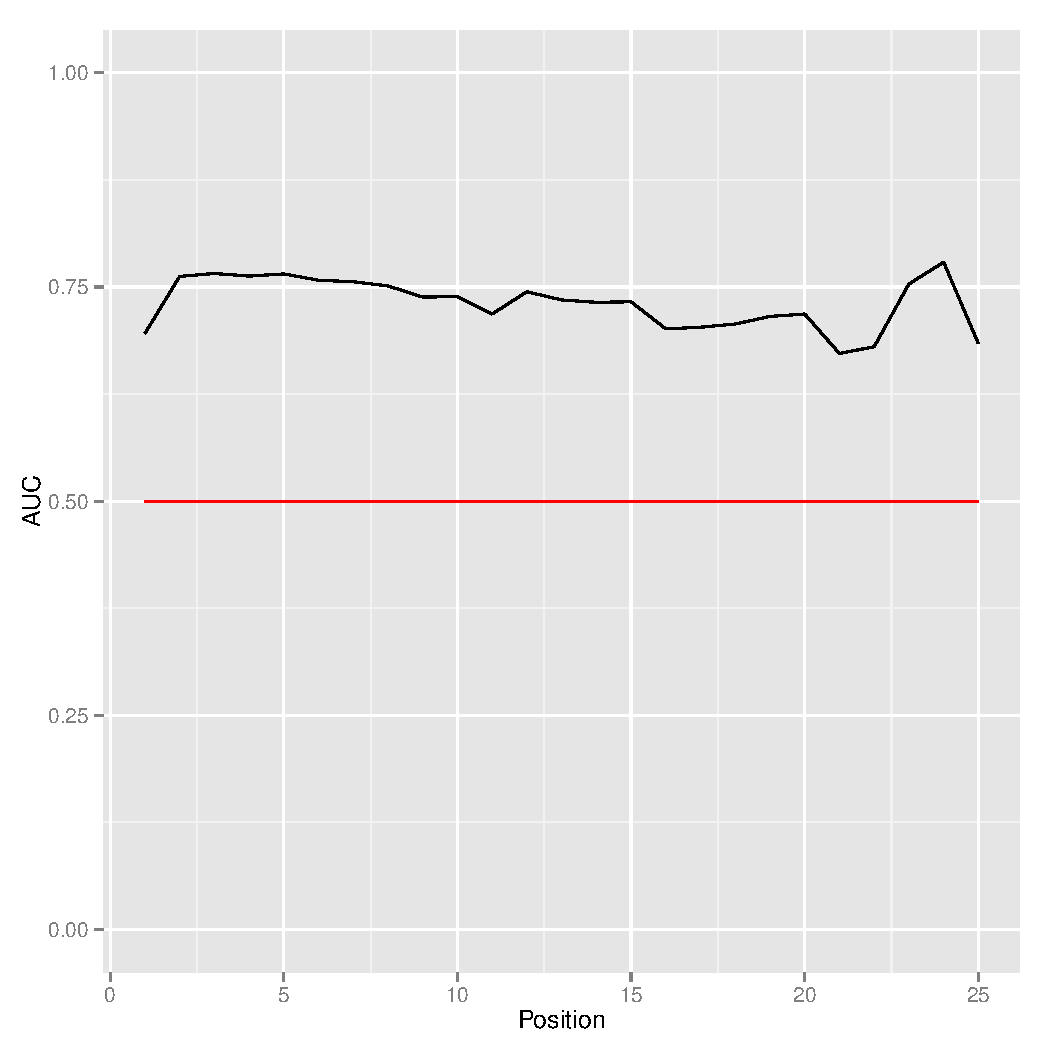
\includegraphics[scale=0.3]{auc.pdf}
\end{frame}

\subsection{Sequential Pattern Mining}

\begin{frame}\frametitle{Häufige Sequenzen in konvertierten und nicht-konvertierten Funnels}
	\centering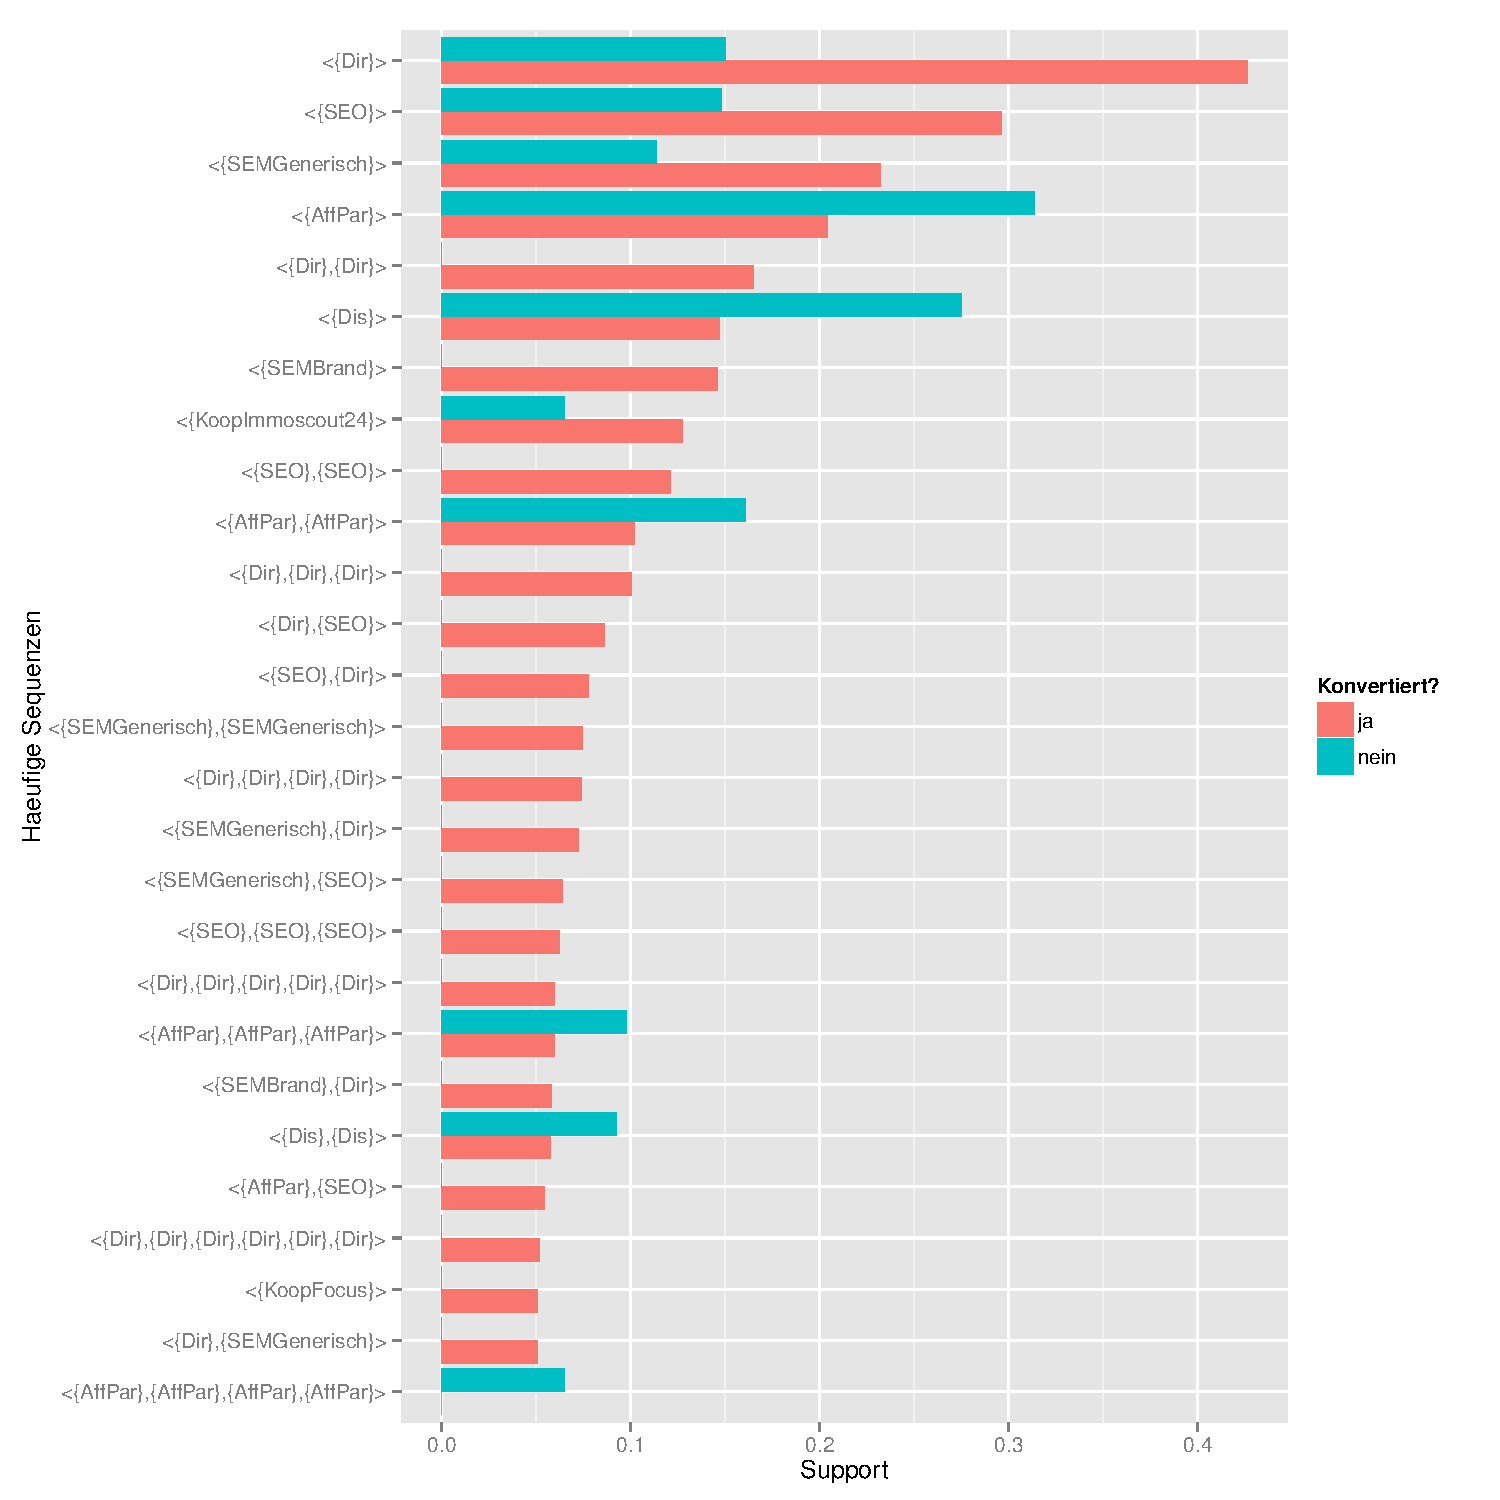
\includegraphics[scale=0.3]{spm_all.pdf}
\end{frame}

\begin{frame}\frametitle{Nur Funnels mit $funnelLength \geq 15$}
	\centering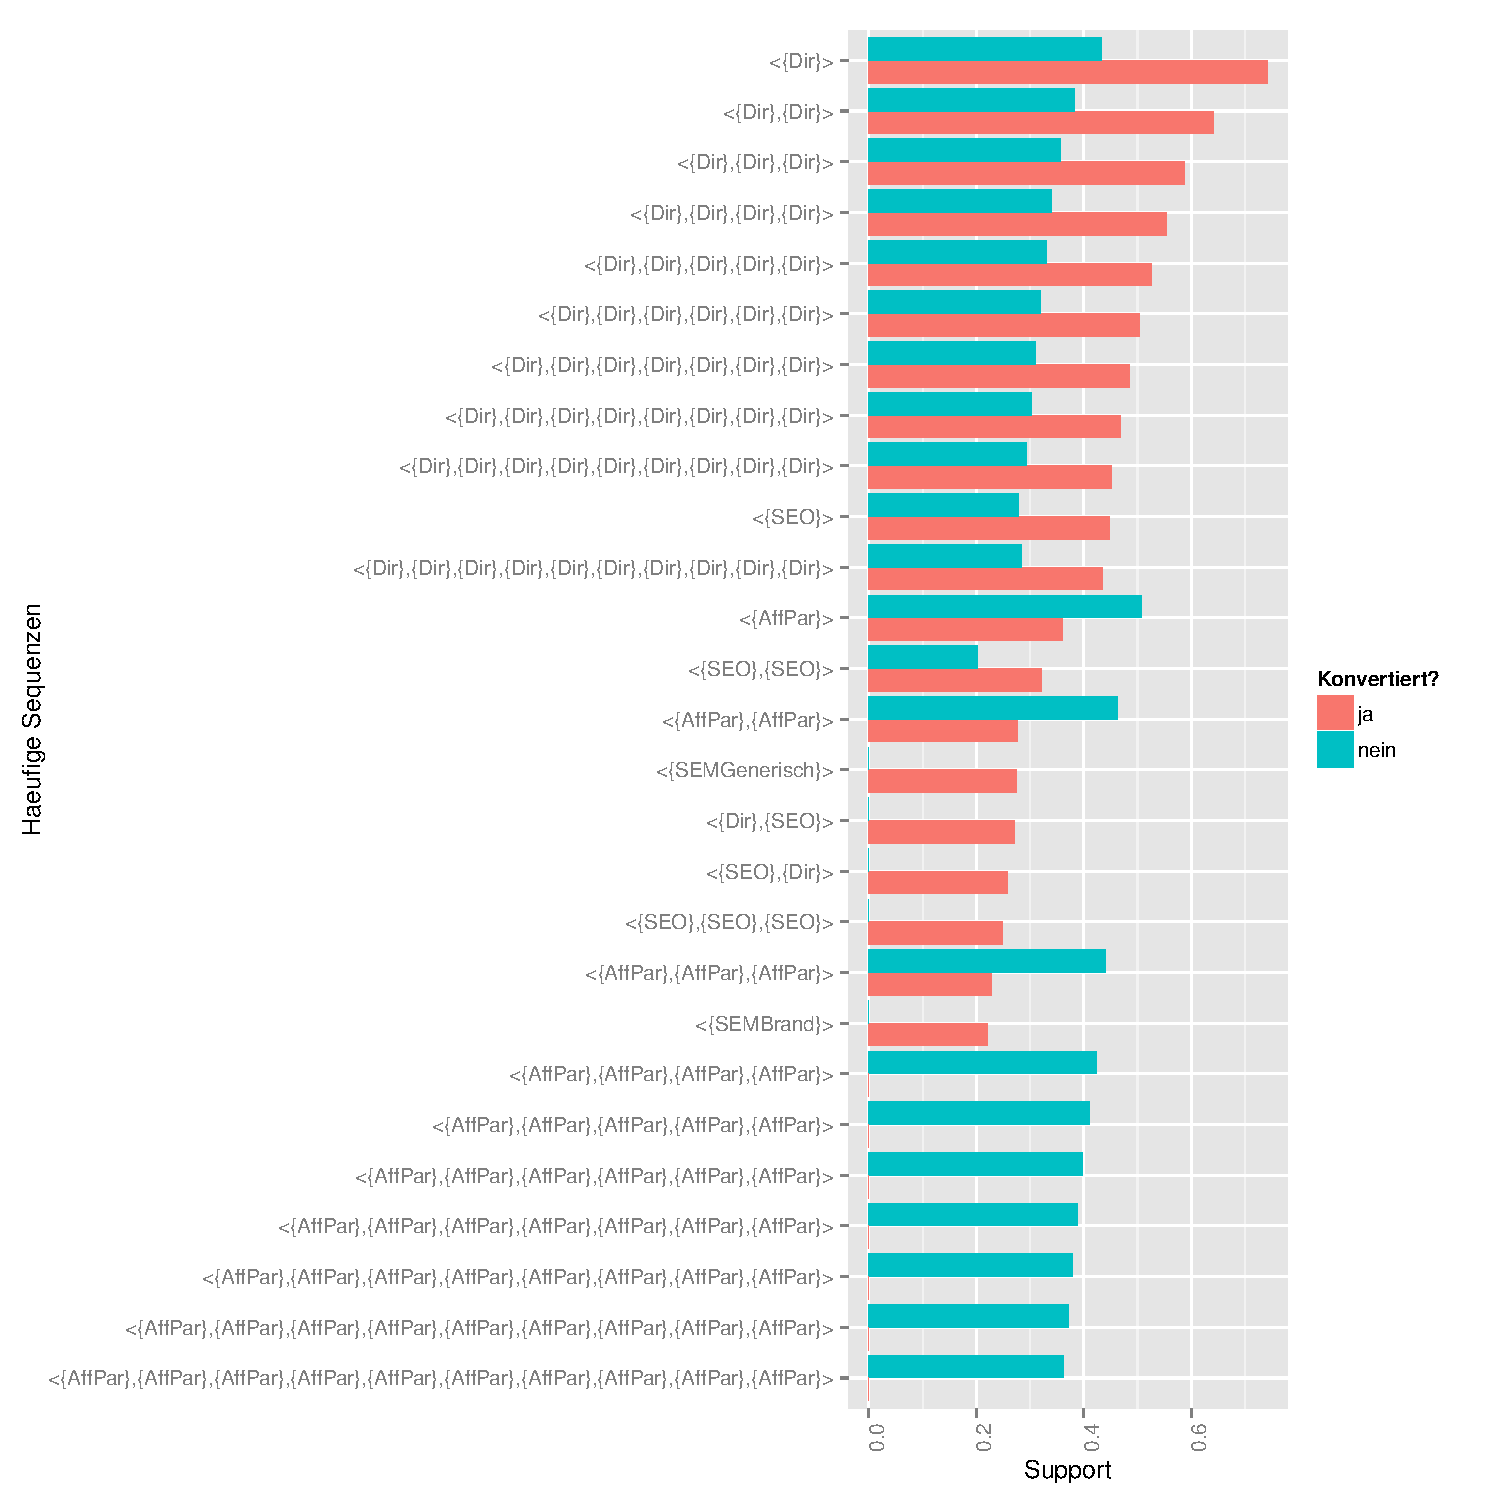
\includegraphics[scale=0.3]{spm_min15.pdf}
\end{frame}

\subsection{Visualisierung anhand eines Netzwerkes}

\begin{frame}\frametitle{Relative Ausgänge}
	\centering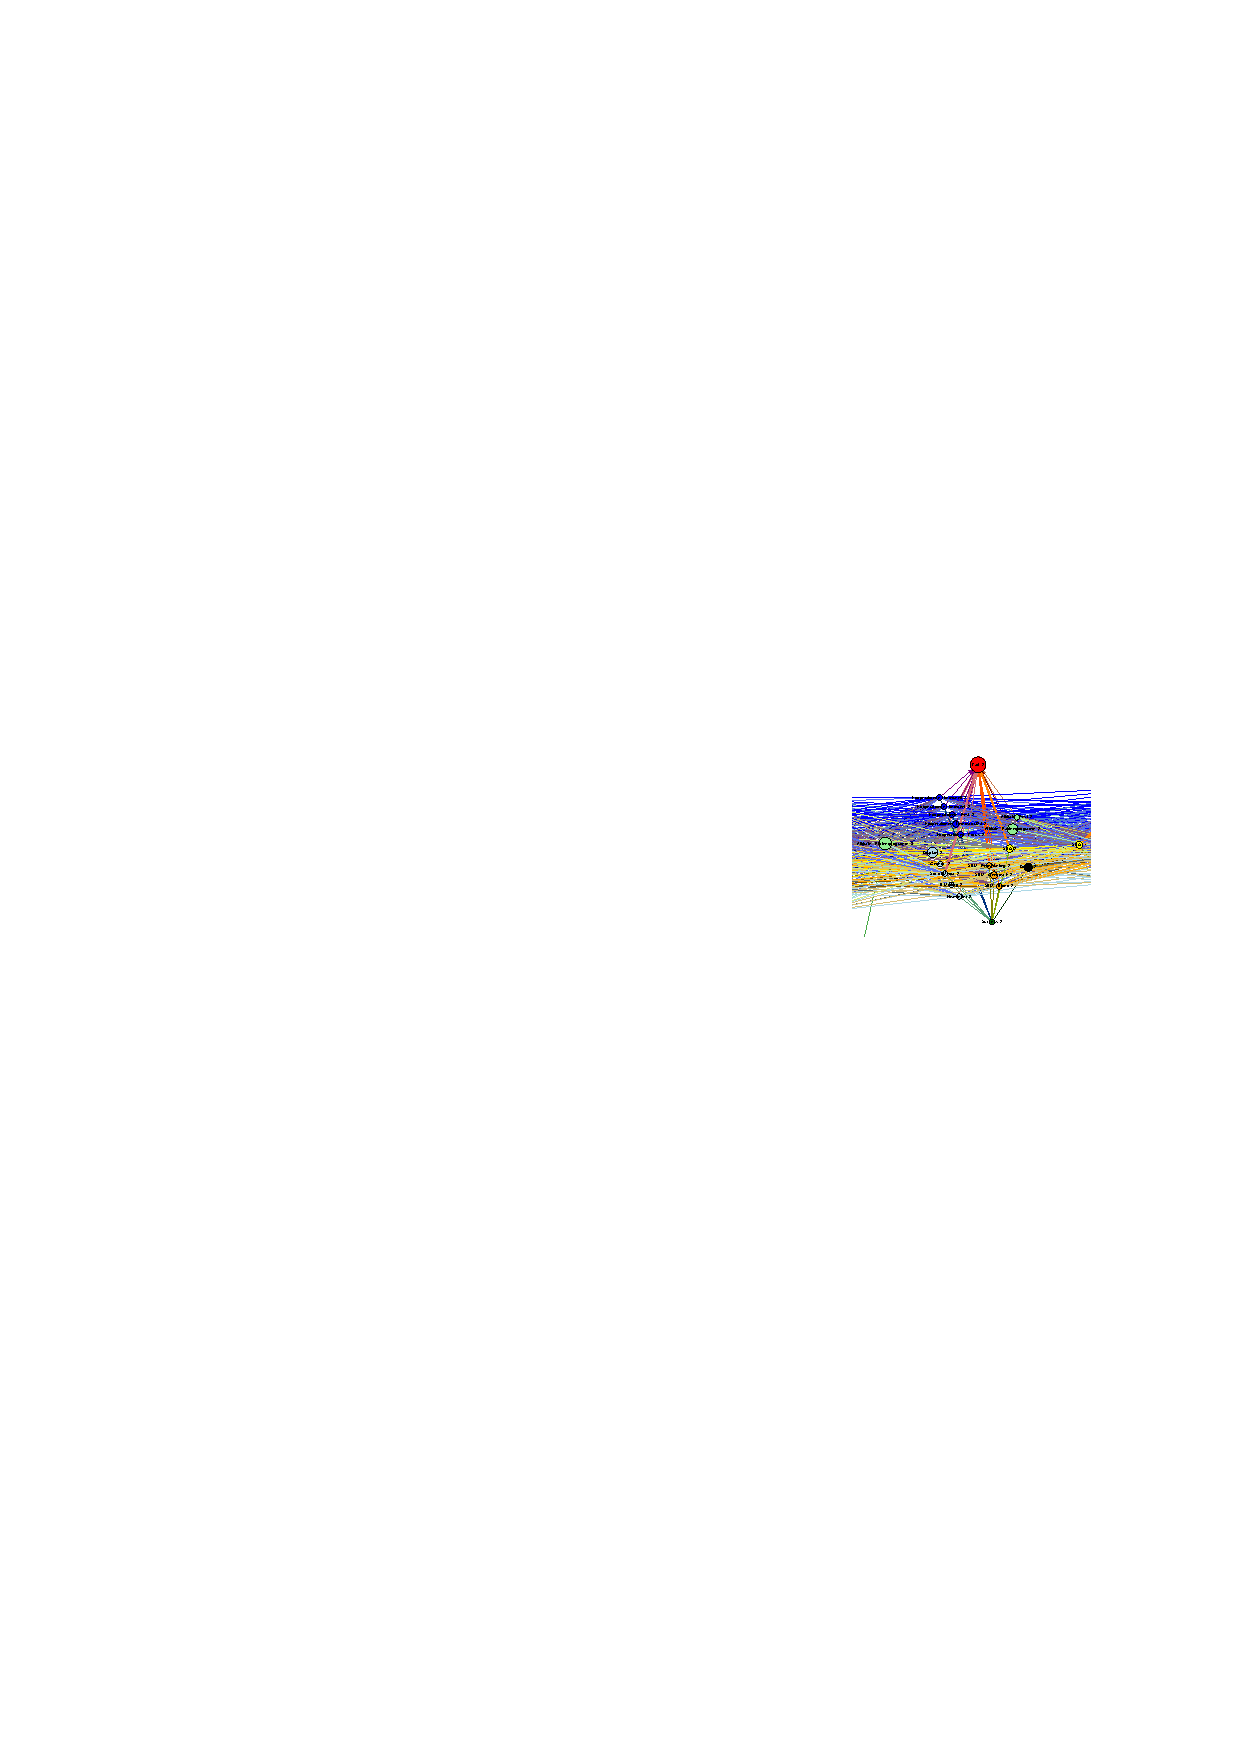
\includegraphics[scale=0.3]{out_labels.pdf}
\end{frame}

\begin{frame}\frametitle{Relative Ausgänge mit Filter $0.02$}
	\centering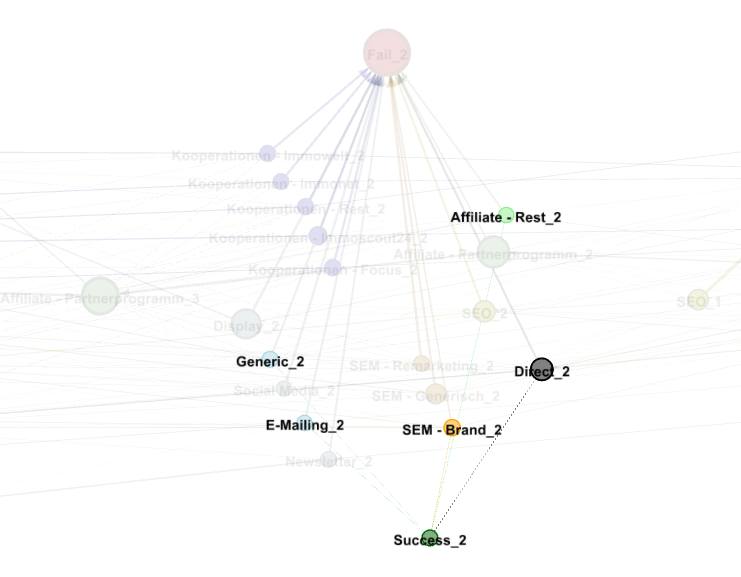
\includegraphics[scale=0.3]{out_filter_2_succ.png}
\end{frame}

\begin{frame}\frametitle{Relative Ausgänge mit Filter $0.5$}
	\centering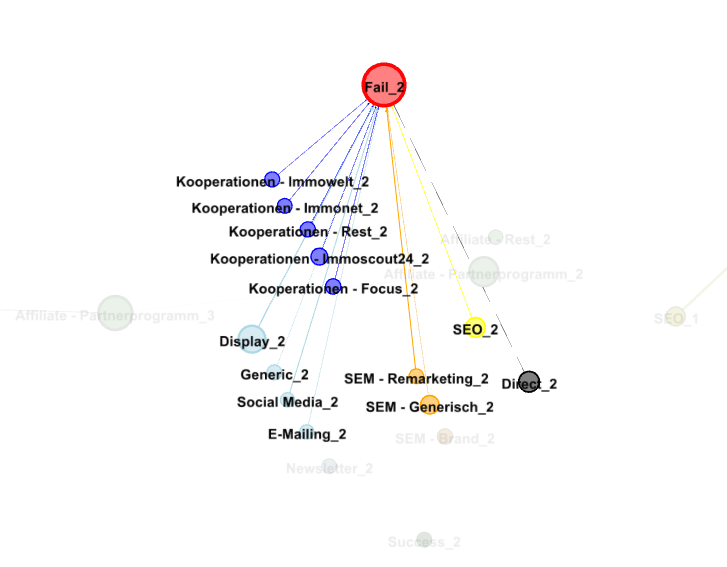
\includegraphics[scale=0.3]{out_filter_50_fail.png}
\end{frame}

\begin{frame}\frametitle{Relative Eingänge}
	\centering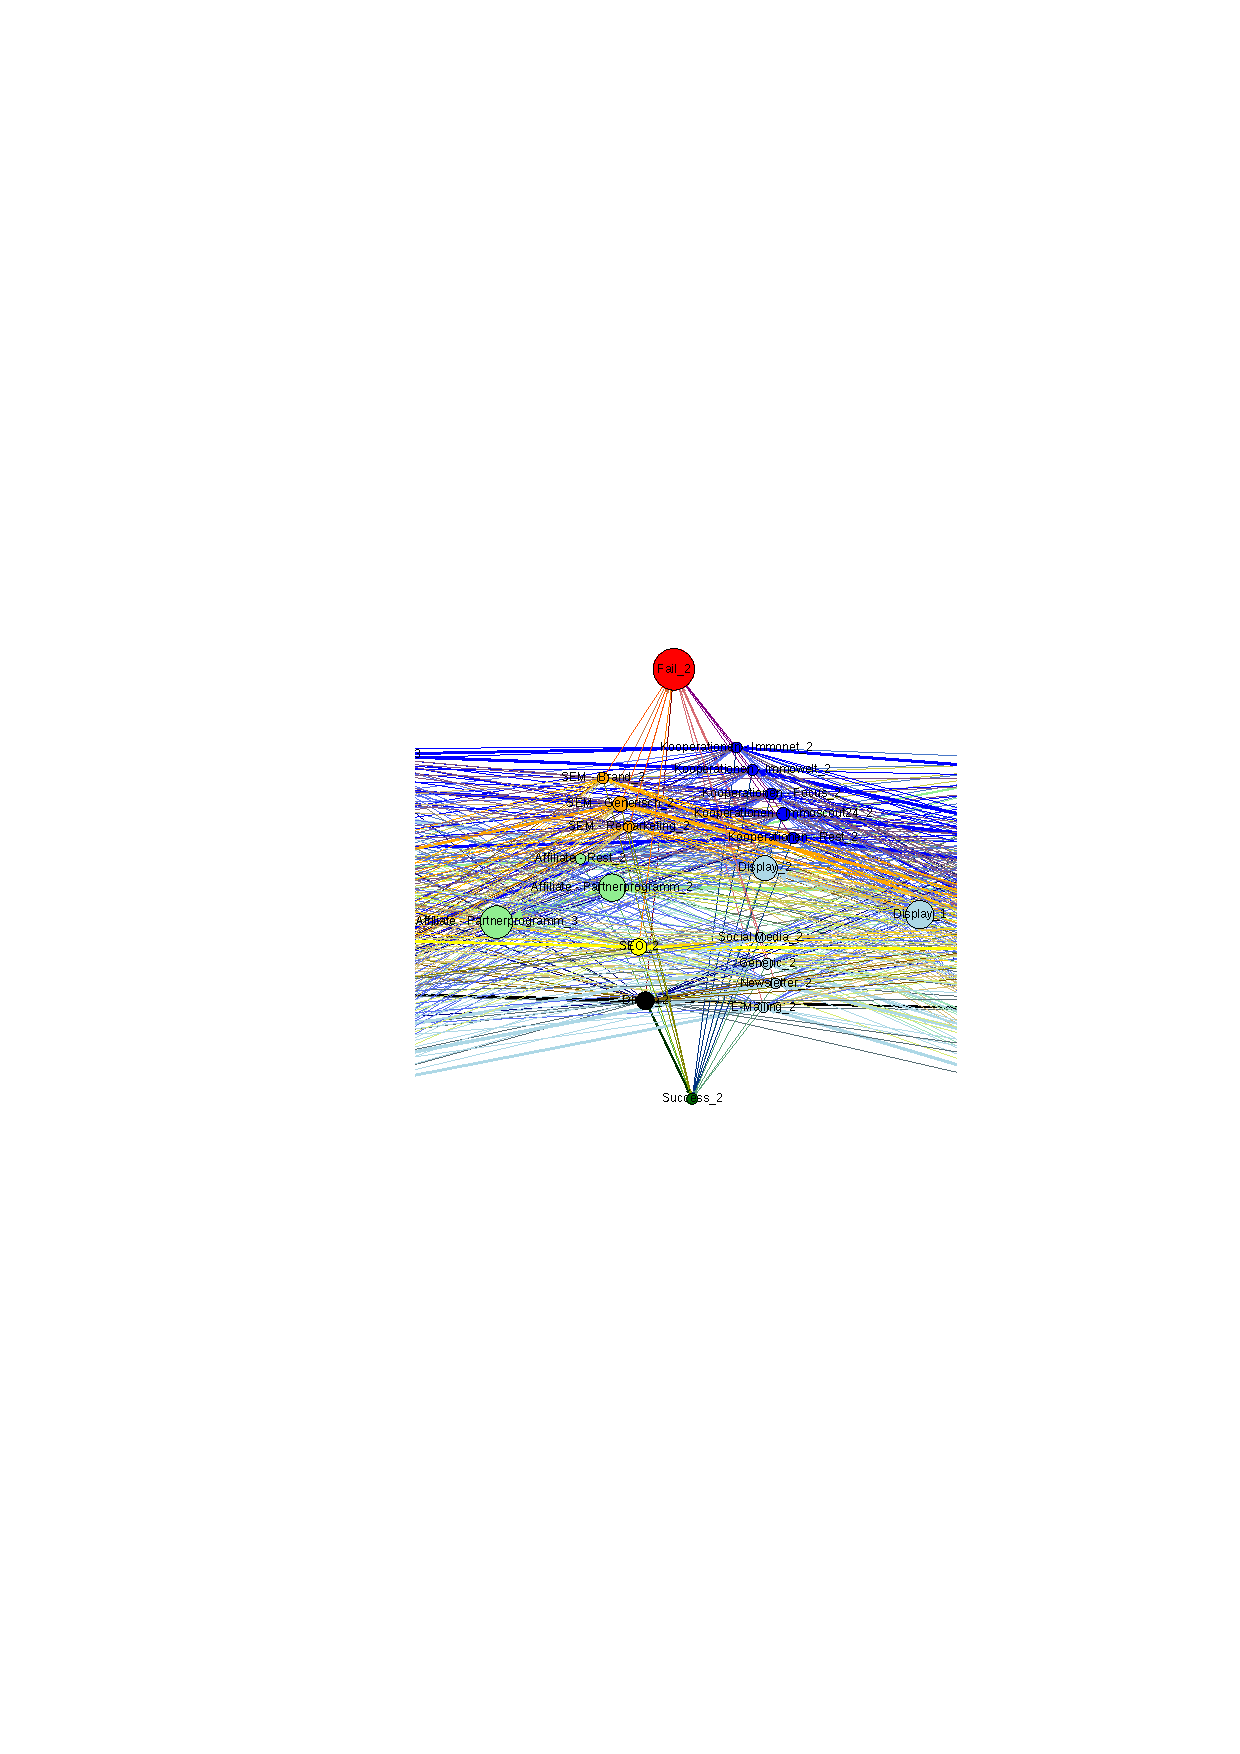
\includegraphics[scale=0.3]{in_labels.pdf}
\end{frame}

\begin{frame}\frametitle{Relative Eingänge mit Filter $0.1$}
	\centering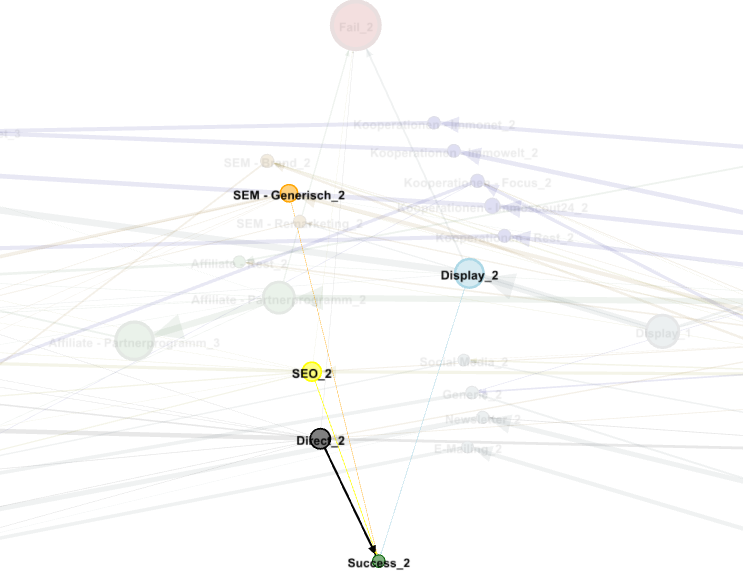
\includegraphics[scale=0.3]{in_filter_10_succ.png}
\end{frame}

\begin{frame}\frametitle{Relative Eingänge mit Filter $0.1$}
	\centering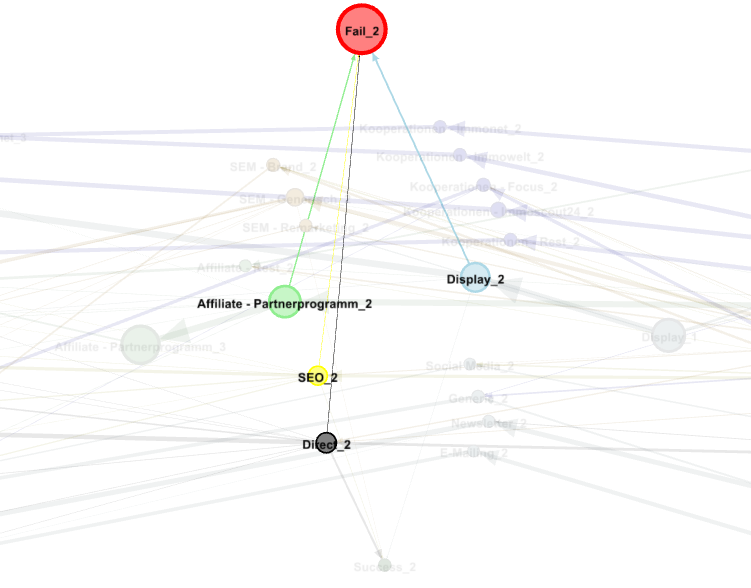
\includegraphics[scale=0.3]{in_filter_10_fail.png}
\end{frame}

%\begin{frame}
	%\begin{columns}
		%\column{7cm}
			%\includegraphics[scale=0.43]{ltwBothMAE.pdf}
		%\column{4cm}
			%\begin{itemize}
				%\item Linearer Zusammenhang zwischen MAE \& Anzahl Bezirke
				%\item kein klarer Unterschied zwischen Cluster \& Strat. Cluster erkennbar
			%\end{itemize}
	%\end{columns}
%\end{frame}